\documentclass[12pt]{article}

% Solutions toggle
\newif\ifsolutions
\solutionsfalse
%% \solutionstrue

% ASSIGNMENT NUMBER
\newcommand{\hwnumber}{8}
\newcommand{\booksection}{}
\newcommand{\duedate}{}
% -------------

%%% Packages
\usepackage[margin=1in, footskip=24pt, headheight=24pt]{geometry}
\usepackage{amsmath, amssymb, amsthm, graphicx}
\usepackage{mathtools}
\DeclarePairedDelimiter\ceil{\lceil}{\rceil}
\DeclarePairedDelimiter\floor{\lfloor}{\rfloor}
\usepackage[colorlinks, urlcolor=blue]{hyperref}
\usepackage{color}
\usepackage{comment}
\usepackage{enumerate}
\usepackage{lastpage}
\usepackage{multirow, multicol}
\usepackage{tikz}
\usetikzlibrary{matrix,decorations.text,decorations.pathmorphing,decorations.markings,arrows,calc,shapes.geometric,patterns,shadows,intersections,decorations.markings,decorations.pathreplacing,decorations.pathreplacing,backgrounds,angles,quotes}
\usepackage{pgfplots}
\pgfplotsset{compat=1.16}

\usepackage{fancyhdr}

\pagestyle{fancy}
%% \renewcommand{\familydefault}{\sfdefault}

\newcommand{\R}{\mathbb{R}}
\newcommand{\ddx}{\frac{d}{dx}}

\global\long\def\V#1{\boldsymbol{#1}} %vector
\global\long\def\M#1{\boldsymbol{#1}} %matrix

\global\long\def\D#1{\Delta#1} %\D{t} for time step size
\global\long\def\d#1{\delta#1} %\d{t} for small increment

\global\long\def\norm#1{\left\Vert #1\right\Vert }
\global\long\def\abs#1{\left|#1\right|}

\global\long\def\grad{\M{\nabla}}
\global\long\def\av#1{\left\langle #1\right\rangle }

% HEADER MACROS
\newcommand{\term}{Spring 2022 \& 2023}
\newcommand{\coursename}{Intro Math Modeling}
\newcommand{\coursenumber}{MATH-UA 251}
\newcommand{\course}{\coursename \ (\coursenumber)}

\fancyhead[RO]{\term}
\fancyhead[LO]{\course}
% -------------

%%% Theorem Styles
\theoremstyle{definition}
\newtheorem{ex}{Exercise}

%%%%%%%%%%%%%%%%%%%%%%%% Solutions %%%%%%%%%%%%%%%%%%%%%%%%%%%%%
% \begin{solution} and \begin{answerspace} must be at the beginning of the line.
% Doesn't work inside the \myversions command. Use if statements instead.
% No underscores in comment names

\ifsolutions
\newenvironment{solution}{\color{blue}}{} \excludecomment{answerspace} \newenvironment{notes}{\color{red} \noindent Grading Notes:}{}
\else
\excludecomment{notes} \excludecomment{solution} \includecomment{answerspace} 
\fi
%%%%%%%%%%%%%%%%%%%% End Solutions %%%%%%%%%%%%%%%%%%%%%%%e}


\begin{document}
% HEADER
\begin{center}
%% \ifsolutions
%%   \textbf{\Large Homework \hwnumber\ - \booksection\ (Solutions)}\\
%% \else
%%   \textbf{\Large Homework \hwnumber\ - \booksection}\\
%% \fi
\ifsolutions
  \textbf{\Large Homework \hwnumber\ (Solutions)}\\
\else
  \textbf{\Large Homework \hwnumber}\\
\fi
\vspace{12pt}
Due date: someday, sometime! \duedate

Submit on NYU Brightspace.
\end{center}

%% \noindent Please give complete, well-written solutions to the following exercise. Provide sufficient justification and explanation for a classmate who has not worked on the exercise to understand your solution.


\begin{ex}

  [35 pts] Consider a spherical pendulum of mass $m$ and radius $a$ connected to an anchor with a weight-less rod of length $\ell$ (cf. Figure below). Note that the dimensions of the sphere matter (not a simple point particle) and the total distance between the center of the sphere to the anchor point is $a+\ell$.

  In class, we have calculated $I_0$, the moment of inertia for a sphere about an axis passing through its center of mass. Use the parallel axis theorem to find the moment of inertia about the anchor point. The only torque on the sphere around the anchor point is due to gravity. Use this torque and the definition of angular momentum to find the equation of motion for this pendulum. Show that the obtained differential equation simplifies to that of a simple pendulum (with a point mass) as $a/\ell\to0$.

\begin{figure}[!h]
\begin{center}
  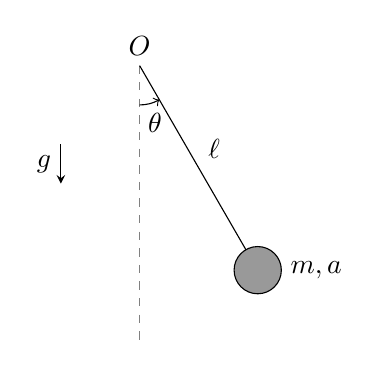
\begin{tikzpicture}
    \pgfmathsetmacro{\myAngle}{30}
    \coordinate (centro) at (0,0);
    \node[anchor=south] at (centro) {$O$};
    \draw[dashed,gray,-] (centro) -- ++ (0,-3.5) coordinate (mary);
    \draw[] (centro) -- ++(270+\myAngle:3) coordinate (bob);
    \pic [draw, ->, "$\theta$", angle eccentricity=1.5] {angle = mary--centro--bob};
    \node[anchor=south west] at ($(centro)!0.5!(bob)$) {$\ell$};
    \filldraw [fill=black!40,draw=black] (bob) circle[radius=0.3] node[anchor=west] {$\;\;\;m,a$};
    \coordinate (grav) at (-1,-1);
    
    \pgfmathsetmacro{\al}{0.5};
    \draw[->,>=stealth] (grav) --++ (0,-\al);
    \node[anchor=east] at ($(grav)+(0,-0.5*\al)$) {$g$};

\end{tikzpicture}
\end{center}
\end{figure}

\begin{solution}
  We showed in class that
  $$I_0=\tfrac{2}{5}ma^2.$$
  Parallel axis theorem gives the moment of inertia about the anchor point:\textcolor{purple}{
  $$I=I_0+m(\ell+a)^2=m\left(\tfrac{2}{5}a^2+(\ell+a)^2\right).$$}%
  The equation of motion in vector form can be written as
  $$\frac{d\V{L}}{dt}=\V{\tau},$$
  where $\V{\tau}$ is the torque due to gravity:
  $$\V{\tau}=\V{R}\times\V{W},$$
  with $\V{R}$ and $\V{W}$ as the center of mass and weight vectors. The magnitude of the torque is $\tau=(\ell+a)mg\sin{\theta}$ and it is in the negative $z$ direction (pointed into the plane) by the right hand rule:
  $$\frac{dL_z}{dt}=-(\ell+a)mg\sin(\theta).$$
  Finally, we use $L_z=I\dot{\omega}_z=I\ddot{\theta}$ to have\textcolor{purple}{
    $$I\ddot{\theta}=-(\ell+a)mg\sin(\theta).$$}%

  To analyze the system when $a/\ell\to0$, start by substituting for $I$:
  \begin{align*}
    &m\left(\tfrac{2}{5}a^2+(\ell+a)^2\right)\ddot{\theta}=-(\ell+a)mg\sin(\theta)\\
    \Rightarrow& m(\ell+a)^2\left(\frac{2}{5}\left(\frac{a}{\ell+a}\right)^2+1\right)\ddot{\theta}=-(\ell+a)mg\sin(\theta)\\
    \Rightarrow& \left(\frac{2}{5}\left(\frac{a/\ell}{1+a/\ell}\right)^2+1\right)\ddot{\theta}=-\frac{1/\ell}{1+a/\ell}g\sin(\theta).
  \end{align*}
  Now let $a/\ell\to 0$ to obtain\textcolor{purple}{
  $$\ddot{\theta}=-\frac{g}{\ell}\sin(\theta).$$}%
\end{solution}
\end{ex}

\begin{ex}

  [30 pts] Consider a physical pendulum as shown in figure below. A thin disk of mass $m$ and radius $a$ is anchored at point $O$ to an axis ($z$, perpendicular to the plane) at a distance $\ell$ away from its center of mass. (Imagine that a thin stick has pierced the disk at point $O$.) The disk can freely rotate about the anchor point (no friction). Neglecting the mass(area) loss due to the anchor, derive the differential equation of motion for the disk.
  
\begin{figure}[!h]
\begin{center}
  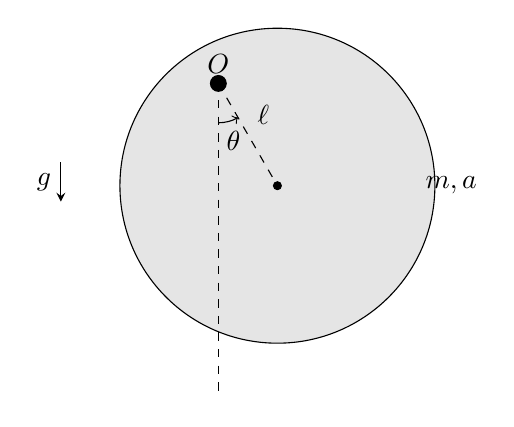
\begin{tikzpicture}
    \pgfmathsetmacro{\myAngle}{30}
    \coordinate (centro) at (0,0);
    \node[anchor=south] at (centro) {$O$};
    \draw[dashed,-] (centro) -- ++ (0,-4) coordinate (mary);
    \draw[dashed] (centro) -- ++(270+\myAngle:1.5) coordinate (bob);
    \pic [draw, ->, "$\theta$", angle eccentricity=1.5] {angle = mary--centro--bob};
    \node[anchor=south west] at ($(centro)!0.5!(bob)$) {$\ell$};
    \begin{scope}[on background layer]
      \filldraw [fill=black!10,draw=black] (bob) circle[radius=2] node[anchor=west] {$\qquad\qquad\quad m,a$};
    \end{scope}
    \filldraw [fill=black,draw=black] (bob) circle[radius=0.05];
    \filldraw [fill=black,draw=black] (centro) circle[radius=0.1];
    \coordinate (grav) at (-2,-1);
    
    \pgfmathsetmacro{\al}{0.5};
    \draw[->,>=stealth] (grav) --++ (0,-\al);
    \node[anchor=east] at ($(grav)+(0,-0.5*\al)$) {$g$};

\end{tikzpicture}
\end{center}
\end{figure}

\begin{solution}
  The solution procedure is very similar to that of the previous problem. We have the moment of inertia of a disk about its center:
  $$I_0=\tfrac{1}{2}ma^2.$$
  Therefore, one can find $I$, the moment of inertia about the anchor point $O$ by the parallel axis theorem:\textcolor{purple}{
    $$I=I_0+m\ell^2=m\left(\tfrac{1}{2}a^2+\ell^2\right).$$}%
  The torque due to gravity is
  $$\V{\tau}=\V{R}\times\V{W}=-\ell mg\sin{\theta}\hat{\V{k}},$$
  where $\hat{\V{k}}$ is the unit vector in the $z$ direction. Hence, the equation of motion can be written as\textcolor{purple}{
  $$\frac{dL_z}{dt}=I\ddot{\theta}=-\ell mg\sin(\theta).$$}%
\end{solution}
\end{ex}

\begin{ex}

  [35 pts] Consider a pulley system as shown in figure below. Assume that the rope is weightless and it does not slip on the pulley, and the effect of the massive pulley with mass $M$ and radius $R$ is \textbf{NOT} negligible. Find the acceleration $a$ of the arrangement. Start by writing the equations of motion for $m_1$ and $m_2$, and the pulley. Hint: you might find the yo-yo problem helpful!

\begin{figure}[!h]
\begin{center}
  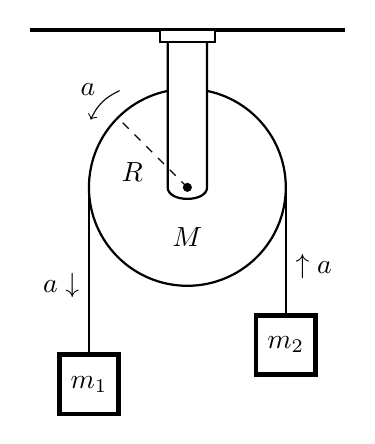
\begin{tikzpicture}
    \pgfmathsetmacro{\l}{2};
    \pgfmathsetmacro{\dx}{0.25};
    \pgfmathsetmacro{\h}{2};
    \pgfmathsetmacro{\basex}{0.35};
    \pgfmathsetmacro{\basey}{0.15};
    \pgfmathsetmacro{\R}{1.25};
    \pgfmathsetmacro{\Rl}{2};
    \pgfmathsetmacro{\Ll}{2.5};
    \pgfmathsetmacro{\X}{0.75};
    \coordinate (T) at ($(0,0) + (0.5*\l,0)$);
    \coordinate (B) at ($(T) + (0,-\h)$);
    \draw[ultra thick] ($(T) + (-\l,0)$) --++ (2*\l,0);
    \draw [thick] (B) circle[radius=\R];
    \path[draw,fill=white,thick] ($(T) + (\dx,0)$) to ($(B) + (\dx,0)$) to [bend left=90] ($(B) + (-\dx,0)$) to ($(T) + (-\dx,0)$);
    \filldraw[thick,fill=white] ($(T) + (-\basex,0)$) rectangle ++(2*\basex,-\basey);
    \filldraw [fill=black,draw=black] (B) circle[radius=0.05];

    \coordinate (R) at ($(B) + (\R,0)$);
    \coordinate (L) at ($(B) + (-\R,0)$);
    \coordinate (RM) at ($(R) + (0,-\Rl)$);
    \coordinate (LM) at ($(L) + (0,-\Ll)$);
    \draw[thick] (R) -- ($(RM) + (0,0.5*\X)$);
    \draw[thick] (L) -- ($(LM) + (0,0.5*\X)$);
    \draw[ultra thick] ($(RM) + (-0.5*\X,0.5*\X)$) rectangle ++(\X,-\X);
    \draw[ultra thick] ($(LM) + (-0.5*\X,0.5*\X)$) rectangle ++(\X,-\X);
    \node at (RM) {$m_2$};
    \node at (LM) {$m_1$};
    \node[anchor=west] at ($(R)+(0,-0.5*\Rl)$) {$\uparrow a$};
    \node[anchor=east] at ($(L)+(0,-0.5*\Ll)$) {$a\downarrow$};

    \node[] at ($(B)+(0,-0.5*\R)$) {$M$};
    \draw[dashed] (B) --++(135:\R) coordinate (ROT);
    \node[anchor=north east] at ($(B)!0.5!(ROT)$) {$R$};

    \pgfmathsetmacro{\dtheta}{20};
    \path[] (B) --++(135-0.5*\dtheta:1.2*\R) coordinate (i);
    \path[] (B) --++(135+0.5*\dtheta:1.2*\R) coordinate (ii);
    \path[draw,->] (i) to [bend right=\dtheta] (ii);
    \node[anchor=south east] at ($(i)!0.5!(ii)$) {$a$};
    
    
\end{tikzpicture}
\end{center}
\end{figure}

\begin{solution}
  The equations of motion for the masses $m_1$ and $m_2$ can be expressed as\textcolor{purple}{
  \begin{align}
    m_1a&=m_1g-T_1,\label{Eq:m1}\\
    m_2a&=T_2-m_2g,\label{Eq:m2}
  \end{align}}%
  where $T_1$ and $T_2$ are the rope tensions at $m_1$ and $m_2$ connections, respectively. We use angular momentum to write the equation of motion for the pulley:
  $$\frac{dL}{dt}=I\frac{d\omega}{dt}=\tau=RT_1-RT_2.$$
  Here $I=\tfrac{1}{2}MR^2$ and we used the right hand rule to find the sign of the torques due to the rope tensions on the left and right sides of the pulley. From the relation between linear velocity and angular velocity, i.e.,
  $$v=R\omega\Rightarrow R\frac{d\omega}{dt}=\frac{dv}{dt}=a,$$
  we find\textcolor{purple}{
  \begin{equation}
    Ia=R^2(T_1-T_2).
    \label{Eq:M}
  \end{equation}}%
  We can now solve \eqref{Eq:m1}--\eqref{Eq:M} for $a$. From \eqref{Eq:m1} and \eqref{Eq:m2} we find
  $$T_1-T_2=-(m_1+m_2)a+(m_1-m_2)g.$$
  Substituting the above expression into \eqref{Eq:M} yields
  $$Ia=R^2\left[-(m_1+m_2)a+(m_1-m_2)g\right]=-(m_1+m_2)R^2a+(m_1-m_2)R^2g,$$
  which can be solved for $a$ to obtain\textcolor{purple}{
  $$a=\frac{(m_1-m_2)R^2g}{I+R^2(m_1+m_2)}=\frac{(m_1-m_2)g}{\tfrac{1}{2}M+m_1+m_2}.$$}%
\end{solution}

\end{ex}

\begin{ex}

  [will not be graded] A spaceship hangs motionless in space at a distance $\ell$ from the center of a planet of mass $M$ and radius $R$. The ship fires an instrument package of mass $m$ with initial speed $v_0$ as shown in the sketch below. Find a formula for the angle $\theta$ for which the package will graze the surface of the planet. Ignore the gravitational pull from the spaceship. As a consistency check, discuss if your formula gives reasonable results when there is no gravitational pull from the planet.

\begin{figure}[!h]
\begin{center}
  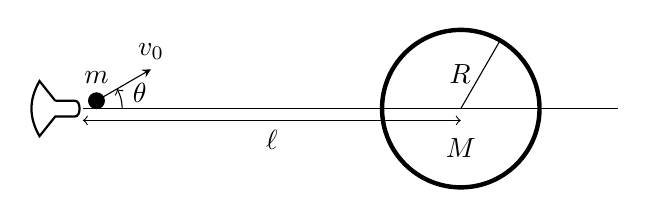
\begin{tikzpicture}
    \pgfmathsetmacro{\l}{5};
    \pgfmathsetmacro{\R}{1};
    \pgfmathsetmacro{\aS}{0.35};
    \pgfmathsetmacro{\dx}{0.15};
    \pgfmathsetmacro{\bS}{0.2};
    \pgfmathsetmacro{\cS}{0.1};
    
    \coordinate (S) at (0,0);
    \coordinate (P) at ($(S)+(\l,0)$);
    \coordinate (Sshift) at ($(S)+(2*\cS,0)$);
    \draw[] (Sshift) -- ($(P)+(2*\R,0)$);
    \draw[ultra thick,draw=black] (P) circle[radius=\R];
    \draw[] (P) --++ (60:\R) coordinate (Surface);
    \node[anchor=east] at ($(P)!0.5!(Surface)$) {$R$};
    \node[] at ($(P)+(0,-0.5*\R)$) {$M$};
    
    \path[draw,thick] ($(S)+(-\dx,0.5*\bS)$) to ($(S)+(\cS,0.5*\bS)$) to [bend left=90] ($(S)+(\cS,-0.5*\bS)$) to ($(S)+(-\dx,-0.5*\bS)$) to ($(S)+(-\aS,-\aS)$) to [bend left=30] ($(S)+(-\aS,\aS)$) to ($(S)+(-\dx,0.5*\bS)$);

    \pgfmathsetmacro{\pl}{0.2};
    \path[] (Sshift) --++ (30:\pl) coordinate (Package);
    \path[] (Package) --++ (30:\pl);
    \filldraw[fill=black,draw=black] (Package) circle[radius=0.1];
    \node[anchor=south] at ($(Package)+(0,0.1)$) {$m$};
    \draw[->,>=stealth] (Package) --++ (30:4*\pl) node[anchor=south] {$v_0$}; 
    \pic [draw, ->, "$\theta$", angle eccentricity=1.5] {angle = P--Sshift--Package};

    \pgfmathsetmacro{\yshift}{0.15};
    \draw[<->] ($(Sshift)+(0,-\yshift)$) -- ($(P)+(0,-\yshift)$);
    \node[anchor=north] at ($($(Sshift)+(0,-\yshift)$)!0.5!($(P)+(0,-\yshift)$)$) {$\ell$};
    
\end{tikzpicture}
\end{center}
\end{figure}

\begin{solution}
  We use the conservation laws to solve this problem. Note that the instrument package experiences a central force from the planet. Therefore, the torque due to this force around the center of the planet is zero and the angular momentum is conserved. We also assume that the energy loss due to drag is negligible and, therefore, the energy is conserved. The total energy can be expressed as
  $$E=K+U=\tfrac{1}{2}mv^2-G\frac{mM}{r},$$
  where $K$ and $U$ are the kinetic and potential energy contributions, $v$ is the package velocity, and $r$ is the distance from the center of the planet. At the launching point, the total energy is
  $$E_i=\tfrac{1}{2}mv_0^2-G\frac{mM}{\ell}.$$
  Similarly, at the collision, we have
  $$E_c=\tfrac{1}{2}mv_R^2-G\frac{mM}{R},$$
  where $v_R$ denotes the velocity at the collision (at distance $r=R$ from the center of the planet).

  With the angular momentum, one can write
  $$L_i=-\ell mv_0\sin(\theta),$$
  and
  $$L_c=-Rmv_R.$$
  where we used the fact that at the collision, the package trajectory will be tangent to planet surface. From the conservation of angular momentum we find\textcolor{purple}{
  $$L_i=L_c\Rightarrow v_R=\frac{\ell}{R}v_0\sin(\theta).$$}%
  From the conservation of energy we obtain
  \begin{align*}
    E_i=E_c&\Rightarrow \tfrac{1}{2}mv_0^2-G\frac{mM}{\ell}=\tfrac{1}{2}mv_R^2-G\frac{mM}{R}=\tfrac{1}{2}m\frac{\ell^2}{R^2}v_0^2\sin^2(\theta)-G\frac{mM}{R},\\
    &\Rightarrow GmM\left(\frac{1}{R}-\frac{1}{\ell}\right)=\tfrac{1}{2}mv_0^2\left(\frac{\ell^2}{R^2}\sin^2(\theta)-1\right).
  \end{align*}
  We can solve the final expression for the angle $\sin(\theta)$:
  $$\sin^2(\theta)=\frac{R^2}{\ell^2}\left[1+\frac{2GM}{v_0^2}\left(\frac{1}{R}-\frac{1}{\ell}\right)\right],$$
  and subsequently, the required angle $\theta$:\textcolor{purple}{
    $$\theta=\sin^{-1}\sqrt{\frac{R^2}{\ell^2}\left[1+\frac{2GM}{v_0^2}\left(\frac{1}{R}-\frac{1}{\ell}\right)\right]}.$$}%

  We see that for $G=0$,
  $$\theta=\sin^{-1}\left(\frac{R}{\ell}\right)\Rightarrow \sin(\theta)=\frac{R}{\ell},$$
  which is expected; in the absence of any gravity, the trajectory of the package will be a straight line that connects the launch point to the planet surface tangentially.
\end{solution}
\end{ex}

\noindent\textbf{\textcolor{red}{notes:} }Show all of the steps of your work. Solutions without details of the work and interpretation of the results will not receive full credits. You need to justify all of your assumptions. Unless otherwise specified, no result can be directly taken from the notes or elsewhere.
\end{document}
